% Documentation for front page:
% https://github.com/martinhelso/mnfrontpage


\documentclass[a4paper, british]{memoir}
% Add [final] to remove marginal notes

\usepackage{style}      % Custom style
\usepackage{kantlipsum} % Dummy text

\hypersetup{
	%I think blue works best for the contents section, but red is best for equations and the like.
	colorlinks  = true, %Colours links instead of ugly boxes
	urlcolor    = blue, %Colour for external hyperlinks
	linkcolor   = blue, %Colour of internal links
	citecolor   = red %Colour of citations
}

\setsecnumdepth{subsubsection}

\title{Characterization of cardiac cellular dynamics using Physics-Informed Neural Networks}
% \subtitle{Optional Subtitle}
\author{Bendik Steinsvåg Dalen}

\includeonly
{
    sections/abstract,
    sections/acknowledgements,
    sections/introduction,
    sections/method,
    sections/results,
    sections/discussion,
    sections/conclusion,
    sections/appendixA,
    sections/appendixB,
}

\begin{document}

    \frontmatter        % Folios in Roman numerals, unnumbered chapters.

    \mnfrontpage

    \abstractintoc % Add abstract to Table of Contents  
\abstractnum   % Format abstract like a chapter
               % Remove if abstract should not be on its own page

\begin{abstract}
	%rewrite. this came out quite badly
    Many \textit{in silico} cardiac cellular models have been developed. These have shown much successes in recreating the behaviour of cardiac cell. However historically there's been many problems in fitting these models to data. In this paper/project we attempt a new approach in using physics-informed neural networks to fit. We found that...
\end{abstract}
    \chapter{Acknowledgements}

\kant[2] % Dummy text
\todo[noline]{Rewrite this.}
\kant[3] % Dummy text

    \cleartorecto
    \microtypesetup{protrusion = false}
    \tableofcontents    % Or \tableofcontents*
    \cleartorecto
    \listoffigures      % Or \listoffigures*
    \cleartorecto
    \listoftables       % Or \listoftables*
    \microtypesetup{protrusion = true}

    \mainmatter         % Folios in Arabic numerals, numbered chapters.
    
    \hypersetup{
    	%I think blue works best for the contents section, but red is best for equations and the like.
    	%I made two differnt ones, but that might be a bit cluncy. 
    	linkcolor   = red, %Colour of internal links
    }

    \chapter{Introduction}
\label{sec:intro}





\section{Outline}

The rest of the text is organised as follows:
\begin{description}
    \item[\cref{sec:method}]
    is second to none, with the notable exception of \cref{sec:intro}.
    The main tool introduced here is the employment of unintelligible sentences.

    \item[\cref{sec:results}]
    asserts the basic properties of being the third chapter of a text.
    This section reveals the shocking truth of filler content.

    \item[\cref{sec:discussion}]
    demonstrates how easily one can get to four chapters by simply using
    the \texttt{kantlipsum} package to generate dummy words.
    
    \item[\cref{sec:conslusion}]
    demonstrates how easily one can get to four chapters by simply using
    the \texttt{kantlipsum} package to generate dummy words.

    \item[\cref{sec:first-app}]
    features additional material for the specially interested.

    \item[\cref{sec:second-app}]
    consists of results best relegated to the back of the document,
    ensuring that nobody will ever read it.
\end{description}

    % \part{The First Part}
    
    \chapter{Method}
\label{sec:method}

\subsection{Physics-Informed Neural Networks}

Physics-informed neural networks (PINN) were introduced by M. Raissi et. al (citation here). 
They are neural networks designed to solve partial differential equations. 
Essentially you constrain a neural network using physical laws.

Create a DNN with param $\theta$
Have two training sets, one for the equ and one for BC/IC
Have a loss function that sums the loss from the pde and the bc
Find best $\theta$ that minimizes the loss function

Define a PDE problem, $u_{t}+\mathcal{N}[u]=0, x \in \Omega, t \in[0, T]$
Define $f:=u_{t}+\mathcal{N}[u]$
Approximate $u(t,x)$ with a DNN
$f(x,t)$ is thus a PINN 
Train by minimizing $M S E=M S E_{u}+M S E_{f}$, where $M S E_{u}=\frac{1}{N_{u}} \sum_{i=1}^{N_{u}}\left|u\left(t_{u}^{i}, x_{u}^{i}\right)-u^{i}\right|^{2}$ and $M S E_{f}=\frac{1}{N_{f}} \sum_{i=1}^{N_{f}}\left|f\left(t_{f}^{i}, x_{f}^{i}\right)\right|^{2}$

To implement PINNs we used the package DeepXDE by Lu Lu et. al (citation here). 


\subsection{Systems Biology Informed Deep Learning}

Further complication of a PINN. 
Adds several layers to the NN: Input-scaling layer, Feature layer, and Output-scaling layer.
Used to infer the hidden dynamics of experimentally unobserved species as well as the unknown parameters in the system of equations


\subsection{FitzHugh–Nagumo}

The FitzHugh–Nagumo model is considered one of the simplest cardiac cell models. It has two states and four variables.

\begin{align}\label{eq:fhn}
    &\dot{v}=v-\frac{v^{3}}{3}-w+R I_{\mathrm{ext}} \\
    &\tau \dot{w}=v+a-b w
\end{align}




    \chapter{Results}
\label{sec:results}

    \chapter{Discussion}
\label{sec:discussion}

    \chapter{Conclusion}
\label{sec:conslusion}

    
    % \chapter{The Second Chapter}
\label{sec:second}
\kant[7-11] % Dummy text
    % \chapter{The Third Chapter}
\label{sec:third}
\kant[12-13] % Dummy text
\section{First Section}
\kant[14]    % Dummy text
\section{Second Section}
\kant[15]    % Dummy text
    % \chapter{The Fourth Chapter}
\label{sec:fourth}
\kant[15-19] % Dummy text

    \appendix           % "Chapter" is renamed "Appendix"
    \appendixpage       % Similar to \part*{Appendices}, but appears in TOC.

%    \chapter{Figures and Tables}
\label{sec:first-app}

\section{Figures}
%
%% Todonotes:
%\begin{figure}[hbp]
%    \centering
%    \missingfigure{Insert a picture of the rockfall in Kvam here.}
%    \caption[Rockfall]{Initiation area of the Kvam rockfall.}
%\end{figure}
%
%% Multiple figures in one
%\begin{figure}[htbp]
%    \centering
%    \begin{subfigure}[t]{0.5\linewidth}
%        \centering
%        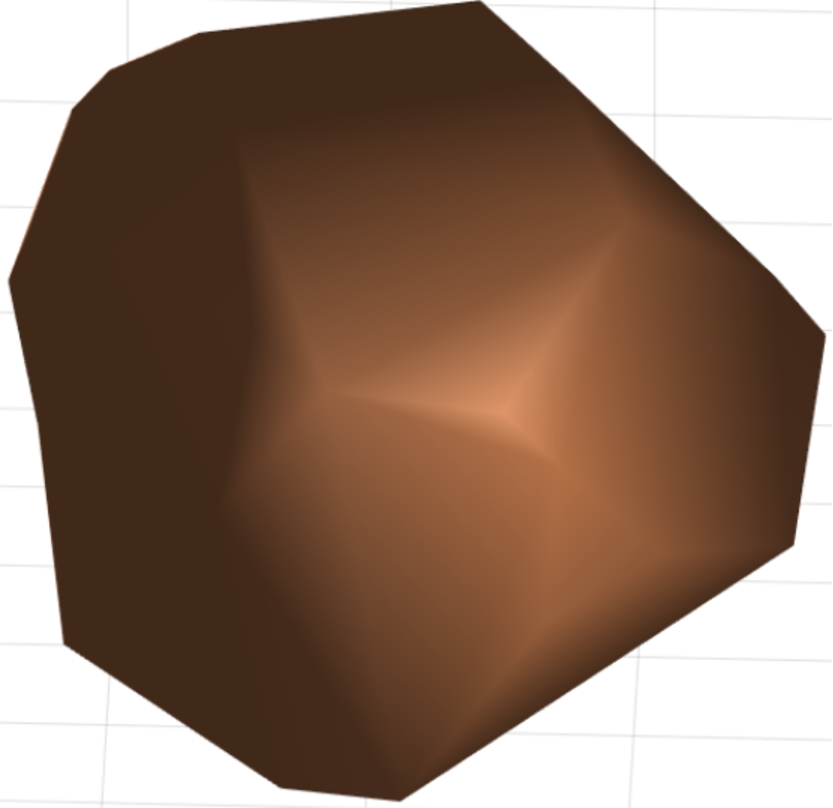
\includegraphics[height = 0.12\textheight]{figures/rock}
%        \caption{Rock simulation.}
%        \label{fig:rock}
%    \end{subfigure}%
%    \begin{subfigure}[t]{0.5\linewidth}
%        \centering
%        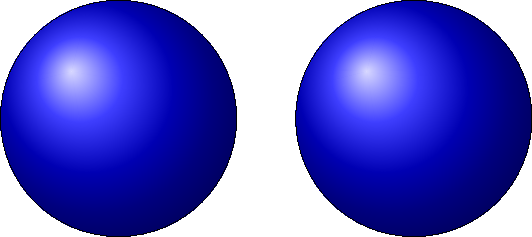
\includegraphics[height = 0.12\textheight]{figures/balls}
%        \caption{Balls.}
%    \end{subfigure}
%    \caption[Subfigures]{A figure with subfigures.}
%    \label{fig:rock-and-balls}
%\end{figure}
%
%\section{Tables}
%\kant[7] % Dummy text
%
%% Math mode for entire column
%\begin{table}[htbp]
%    \caption[Default friction parameters for different types of terrain]
%            {Default friction parameters for different types of terrain \parencite{Bar+11}.}
%    \label{tab:friction-parameters}
%    \centering
%    \begin{tabular}
%        {
%            @{}
%            l
%            >{\(}l<{\)} % Specify that each entry in the column starts with \(
%            >{\(}l<{\)} % and ends with \)
%            >{\(}r<{\)}
%            >{\(}l<{\)}
%            >{\(}l<{\)}
%            @{}
%        }
%        \toprule
%        \textbf{Terrain}
%        &
%        \boldsymbol{\mu_{\min}}
%        &
%        \boldsymbol{\mu_{\max}}
%        &
%        \boldsymbol{\beta_s}
%        &
%        \boldsymbol{\kappa}
%        &
%        \boldsymbol{C_v}
%        \\
%        \midrule
%        Extra soft  & 0.2  & 2    &  50 & 1    & 0.9
%        \\
%        Soft        & 0.25 & 2    & 100 & 1.25 & 0.8
%        \\
%        Medium soft & 0.3  & 2    & 125 & 1.5  & 0.7
%        \\
%        Medium      & 0.35 & 2    & 150 & 2    & 0.6
%        \\
%        Medium hard & 0.4  & 2    & 175 & 2.5  & 0.5
%        \\
%        Hard        & 0.55 & 2    & 185 & 3    & 0.4
%        \\
%        Extra hard  & 0.8  & 2    & 200 & 4    & 0.3
%        \\
%        Snow        & 0.1  & 0.35 & 150 & 2    & 0.7
%        \\
%        \bottomrule
%    \end{tabular}
%\end{table}
%
%% Tablefootnote and multirow:
%\begin{table}[htbp]
%    \centering
%    \caption[Dashes]{Proper dash usage.}
%    \begin{tabular}{@{}ll@{}}
%        \toprule
%        \textbf{Correct}
%        & 
%        \textbf{Incorrect}
%        \\
%        \midrule
%        \( -1 \) 
%        & 
%        -1
%        \\[0.3ex]
%        1--10
%        &
%        1-10
%        \\[0.3ex]
%        Birch--Swinnerton-Dyer\tablefootnote{It is now easy to tell that Birch and Swinnerton-Dyer are two people.} conjecture
%        &
%        Birch-Swinnerton-Dyer conjecture
%        \\[0.3ex]
%        The ball \dash which is blue \dash is round.
%        &
%        \multirow{ 2}{*}{The ball - which is blue - is round.}
%        \\[0.3ex]
%        The ball---which is blue---is round. 
%        &
%        \\
%        \bottomrule
%    \end{tabular}
%\end{table}
%
%% Rotate page
%% Columns with fixed width for paragraph-style formatting
%\begin{landscape}
%    \begin{table}[htbp]
%        \centering
%        \caption[Long, rotated table]{A long, rotated table.}
%        \begin{tabular}
%        {
%            @{}
%            p{0.35\textwidth} % Specify width of column
%            p{0.24\textwidth}
%            p{0.12\textwidth}
%            p{0.35\textwidth}
%            p{0.28\textwidth}
%            @{}
%        }
%            \toprule
%            \bfseries
%            Type of mass movement
%            &
%            \bfseries
%            Location
%            &
%            \bfseries
%            Date
%            &
%            \bfseries
%            Well documented\par
%            (media and/or reports)?
%            &
%            \bfseries
%            Hazard mapping?
%            \\
%            \midrule
%            Landslide in rock
%            &
%            Kvam, Nord-Fron
%            &
%            11/06/16
%            &
%            Yes
%            &
%            Yes (2016, after event)
%            \\
%            Landslide in rock
%            &
%            Voss (Fornestræet)
%            &
%            08/06/16
%            &
%            Yes
%            &
%            No
%            \\
%            Landslide in rock
%            &
%            Matbjøra
%            &
%            15/09/16
%            &
%            Yes
%            &
%            No
%            \\
%            Landslide in rock
%            &
%            Gudvangen
%            &
%            16/07/16
%            &
%            Yes
%            &
%            No
%            \\
%            \midrule
%            Debris flow
%            &
%            Flåklypa, Lom
%            &
%            19/05/16
%            &
%            No
%            &
%            No
%            \\
%            Debris flow
%            &
%            Rindane
%            &
%            26/11/15
%            &
%            Yes
%            &
%            Yes
%            \\
%            Debris flow
%            &
%            Skjeldvik, Odda
%            &
%            26/12/11
%            &
%            Yes
%            &
%            No
%            \\
%            Debris flow
%            &
%            Beisfjord
%            &
%            14/07/12
%            &
%            Yes
%            &
%            No
%            \\
%            \midrule
%            Debris slide
%            &
%            Årsetdalen
%            &
%            09/06/11
%            &
%            Yes
%            &
%            Yes (2015)
%            \\
%            Debris slide
%            &
%            Borga, Romsdalen
%            &
%            26/11/15
%            &
%            Yes
%            &
%            No
%            \\
%            Debris slide
%            &
%            Vatne
%            &
%            15/11/13
%            &
%            Yes
%            &
%            No
%            \\
%            Debris slide
%            &
%            Gjerde, Luster
%            &
%            05/07/15
%            &
%            Yes
%            &
%            No
%            \\
%            Debris slide
%            &
%            Skredestranda
%            &
%            15/11/13
%            &
%            Yes
%            &
%            No
%            \\
%            Debris slide
%            &
%            Berge, Høyanger
%            &
%            26/12/11
%            &
%            Yes
%            &
%            Yes (2014)
%            \\
%            Debris slide
%            &
%            Oldedalen
%            &
%            17/11/13
%            &
%            Yes
%            &
%            No
%            \\
%            \bottomrule
%        \end{tabular}
%    \end{table}
%\end{landscape}
%    \chapter{Computer Code}
\label{sec:second-app}

The following \matlab script produced the simulated rock in \cref{fig:rock}:

\lstinputlisting[language = Matlab]{code/rock.m}

    \backmatter         % Folios in Arabic numerals, unnumbered chapters.

    \printbibliography

\end{document}